\section{Étude expérimentale}
Cette section présente les différents outils utilisés à l'aboutissement de l'application réalisée ainsi que l'architecture de l'application développée.
A partir de l'application développée nous réalisons une étude expérimentale d'un exemple issu de la vie courante, ensuite nous interprétons les résultats expérimentale obtenus par la méthode de redistribution proposée dans ce chapitre.

\subsection{Outils de développement}
Pour la mise en œuvre d’une application de distribution de l'espace d'états et de la vérification formelle, la capacité à monter en charge s’envisage pour pouvoir évoluer de façon fluide en fonction de l'augmentation de la demande des ressources afin qu'une expérimentation soit menée dans les meilleures conditions. Dans ce qui suit nous pressentons les outils nécessaires pour le développement de ce type d'application. \newpage

\subsubsection*{Langage de programmation Java}
\begin{wrapfigure}{r}{0.2\textwidth}
	\vspace{-60pt}
	\begin{center}
		
\includegraphics[width=0.1\textwidth]{img/java}
	\end{center} 
	\vspace{-20pt}
	\vspace{-10pt} 
\end{wrapfigure}
Java est un langage de programmation moderne orientée objet développé par Sun Microsystems (aujourd'hui racheté par Oracle) \citep{java}. Le langage Java permet la programmation parallèle, le développement des applications reparties, l'accès à des bases de données, l'accès à des traitements en d'autres langages. Ainsi, les applications développées sous le langage  Java sont portables sur plusieurs systèmes d’exploitation tels que Unix, Windows, Mac OS ou GNU/Linux. Par contre elles sont plus lourdes à l'exécution (en mémoire et en temps processeur) à cause de sa machine virtuelle.
\subsubsection*{La plateforme JADE}
\begin{wrapfigure}{r}{0.2\textwidth}
	\vspace{-60pt}
	\begin{center}
		
\includegraphics[width=0.3\textwidth]{img/jade}
	\end{center} 
	\vspace{-20pt}
	\vspace{-10pt} 
\end{wrapfigure}
JADE (Java Agent Development Framework) est une plateforme de programmation multi-agent implémentée en Java \citep{jade}. Elle est open-source et distribuée par Telecom Italia sous la licence LGPL. La plateforme héberge un ensemble d’agents, identifiés de manière unique, pouvant communiquer de manière bidirectionnelle avec les autres agents. Ainsi Chaque agent s’exécute dans un conteneur (container) qui lui fournit son environnement d’exécution.
\subsubsection*{IDE IntelliJ}
\begin{wrapfigure}{r}{0.2\textwidth}
	\vspace{-40pt}
	\begin{center}
		
\includegraphics[width=0.1\textwidth]{img/ida}
	\end{center} 
	\vspace{-20pt}
	\vspace{-10pt} 
\end{wrapfigure}
IntelliJ est un environnement de développement intégré (IDE) pour le développement de logiciels. Il propose de nombreux outils pour faciliter le développement dont  l'auto-complétion syntaxique, une vérification d'erreur en live, différents outils de compilation, des outils de debugging avancés, etc. IDE IntelliJ est adapté pour coder en Java, en plus de java plusieurs plugins sont offert pour le développement logiciels.

\subsubsection*{Docker}
\begin{wrapfigure}{r}{0.2\textwidth}
	\vspace{-60pt}
	\begin{center}
		
\includegraphics[width=0.2\textwidth]{img/docker}
	\end{center} 
	\vspace{-20pt}
	\vspace{-10pt} 
\end{wrapfigure}
Docker une plateforme logicielle open source permettant la mise en œuvre de systèmes distribués. Il permet à de multiples applications, tâches de fond et autres processus de s'exécuter de façon autonome sur une seule machine physique ou à travers un éventail de machines isolées. Il a été développé par Solomon Hykes avec les contributions d'Andrea Luzzardi et Francois-Xavier Bourlet  \citep{docker}. Les services ou fonctions de l’application et ses différentes bibliothèques, fichiers de configuration, dépendances et autres composants sont regroupés au sein d'un container. Chaque container exécuté partage les services du système  d’exploitation de la machine physique.

\subsubsection*{Neo4j}
\begin{wrapfigure}{r}{0.2\textwidth}
	\vspace{-20pt}
	\begin{center}
		
\includegraphics[width=0.2\textwidth]{img/neo4j-logo-2015}
	\end{center} 
	\vspace{-20pt}
	\vspace{-10pt} 
\end{wrapfigure}
Neo4j est une base de données graphe \citep{neo4j}, sous licence GPLv3, implémenté en Java et un langage de requête de graphe déclaratif simple et efficace (Cypher). Développée par Neo Technology dans le but d'offrir une structure de stockage dédiées aux  graphes ainsi qu'une parcours des données en utilisant les arcs pour passer d'un nœud à l'autre. De plus, il offre une haute disponibilité des données et le stockage des milliards de nœuds et de relations.			

\subsubsection*{GraphViz}
\begin{wrapfigure}{r}{0.2\textwidth}
	\vspace{-50pt}
	\begin{center}
		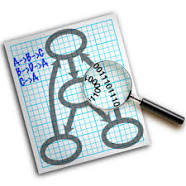
\includegraphics[width=0.2\textwidth]{img/graphviz}
	\end{center}  
\vspace{-20pt}
\vspace{-10pt}  
\end{wrapfigure}
GraphViz (Graph Visualiszation Software) est un ensemble d'outils de visualisation de graphes, créés par les laboratoires de recherche d'AT\&T \citep{graphviz}. Il utilise des fichiers textes suivant le langage $DOT$ pour représenter les données structurées sous forme de graphes. le langage $DOT$ permet  de personnaliser le rendu des graphes par le choix des formes, couleurs et polices de caractères. Ainsi le graphe définie est exporté sous différents formats d'images (FIG, PNG, JPEG, GIF, etc.).




\subsection{Architecture de l'application}

\subsection{Configuration de la mise en œuvre}
Nous avons développé un outil qui génère une structure de Kripke distribuée. L’outil dispose d’un éditeur de graphique pour dessiner et modifier les systèmes analysés à partir d'un réseau de Petri (Figure \ref{apppetrinet}).

L’approche proposée a été implémenter avec le langage de programmation JAVA sur IDE IntelliJ, en utilisant le base de donnée orienté graphe Neo4J pour le stockage de l'espace d'états, le Docker pour l'hébergement de ces bases de données. le framework Java Agent Development est aussi utiliser pour faciliter la communication entre les machines.

\subsection{Expérimentation}